\documentclass[11pt]{article}
\usepackage{amsfonts,amsthm,amsmath,amssymb, hyperref, dsfont, enumitem, bbm}
\usepackage{array}
\usepackage{epsfig}
\usepackage{fullpage}
\usepackage{color}
\usepackage{epigraph}
\renewcommand{\epigraphflush}{center}
\usepackage[framemethod=tikz]{mdframed}
\usepackage{titlesec}
\usepackage{ellipsis}
\usepackage{subcaption}
\usepackage[normalem]{ulem}
\usepackage{todonotes}

\usepackage{tikz}
\usepackage{pgfplots}
\usepackage{clrscode3e,etoolbox}


\titleformat{\chapter}[display]
  {\normalfont\bfseries}{}{0pt}{\Huge}





%%%%%%%%%%%%%%%%%%%%%%%%%%%%%%%%%%%%%%%%%%%%%%%%%%%%%%%%%%%%%%%%%%%%%%
% Structure
%%%%%%%%%%%%%%%%%%%%%%%%%%%%%%%%%%%%%%%%%%%%%%%%%%%%%%%%%%%%%%%%%%%%%%

% Don't put chapter number in section numbers
% \renewcommand*\thesection{\arabic{section}}	% commented out to include chapter number in section numbers

\newcommand{\anchorednote}[2]{ #1 \note{#2} }	% anchored note - needed for latex2edx
\newcommand{\note}[1]{\todo[color=blue!10,
  linecolor=blue!90,size=\small]{\linespread{0.9}\selectfont{#1}\par}}

\usepackage{tcolorbox}
\newtcolorbox{examplebox}{colback=green!5!white}

% \scalebox{1.5}{\begin{tikzpicture}
%   % Put your tikz code here
% \end{tikzpicture}}

\newcommand\question[1]{\vskip0.05in\todo[inline, color=yellow!5]{{\bf
      Study Question:}  #1}} 

\def\myrightmargin{2.0in}

% Make it compact for printing
\renewcommand{\note}[1]{\footnote{#1}}
\def\myrightmargin{1.0in}
\usepackage[left=1in, top=1in, bottom=1in,right=\myrightmargin]{geometry}



%%%%%%%%%%%%%%%%%%%%%%%%%%%%%%%%%%%%%%%%%%%%%%%%%%%%%%%%%%%%%%%%%%%%%%
% Math macros
%%%%%%%%%%%%%%%%%%%%%%%%%%%%%%%%%%%%%%%%%%%%%%%%%%%%%%%%%%%%%%%%%%%%%%

% Use to index over examples

\newcommand\ex[2]{#1^{(#2)}}
% Data sets
\newcommand\data{{\cal D}}
\newcommand\dataTrain{{\cal D}_n}
\newcommand\dataTest{{\cal D}_{n'}}
% Model, hypoth
\newcommand\model{{\cal M}}
\newcommand\hclass{{\cal H}}
% Max likelihood
\newcommand\ml[1]{#1_{\bf ml}}
% Empirical risk min
\newcommand\erm[1]{#1_{\bf erm}}
% Arg max
\newcommand\argmax[1]{{\rm arg}\max_{#1}}
\newcommand\argmin[1]{{\rm arg}\min_{#1}}
% Math
\newcommand{\R}{\mathbb{R}}
% errors
\newcommand{\trainerr}{\mathcal{E}_n}
\newcommand{\testerr}{\mathcal{E}}
% sign
\newcommand{\sign}{\text{sign}}
% 2d vec
\newcommand*{\twodrow}[2]{\begin{bmatrix} #1 & #2 \end{bmatrix}}
\newcommand*{\twodcol}[2]{\begin{bmatrix} #1 \\ #2 \end{bmatrix}}
% norm














\newcommand{\qn}[1]{\textcolor{orange}{Quynh: #1}}




\begin{document}

%% Courtesy: Daniel Spielman, via Madhu Sudan --> Chi-Ning Chou --> Anurag Anshu

\theoremstyle{plain}
\newtheorem{theorem}{Theorem}[section]
\newtheorem{lemma}[theorem]{Lemma}
\newtheorem{example}[theorem]{Example}
\newtheorem{corollary}[theorem]{Corollary}
\theoremstyle{definition}
\newtheorem{definition}[theorem]{Definition}
\newtheorem*{mydefinition}{Definition}
\newtheorem{claim}[theorem]{Claim}
\newtheorem{fact}[theorem]{Fact}
\newtheorem{remark}[theorem]{Remark}
\newtheorem{exercise}[theorem]{Exercise}

%Left and right brackets
\newcommand {\br} [1] {\ensuremath{ \left( #1 \right) }}
\newcommand {\Br} [1] {\ensuremath{ \left[ #1 \right] }}


%Quantum notations
\newcommand {\norm}[1]{{\| #1 \|}}  
\newcommand {\bra} [1] {\ensuremath{ \left\langle #1 \right| }}
\newcommand {\ket} [1] {\ensuremath{ \left| #1 \right\rangle }}
\newcommand {\ketbratwo} [2] {\ensuremath{ \left| #1 \middle\rangle \middle\langle #2 \right| }}
\newcommand {\ketbra} [1] {\ketbratwo{#1}{#1}}
\newcommand{\braket}[2]{\langle#1|#2\rangle}
\newcommand{\Tr}[1]{\mathrm{Tr}\left(#1\right)}
\newcommand{\tr}[2]{\mathrm{Tr}_{#1}\left(#2\right)}
\newcommand{\PE}{\mathrm{PE}}
\newcommand{\EPR}{\mathrm{EPR}}
\newcommand{\CNOT}{\mathrm{CNOT}}
\newcommand{\CZ}{\mathrm{CZ}}

%Generic math symbols
\newcommand {\eps} {\varepsilon}
\newcommand{\tO}{\tilde{O}}
\newcommand{\ind}[1]{\mathrm{Ind}\left(#1\right)}
\newcommand {\id}{\mathds{1}}
\newcommand{\bitn}[1]{\ensuremath{\{0,1\}^{#1}}}
\newcommand{\bitone}{\ensuremath{\{0,1\}}}
\newcommand{\swp}{\mathrm{\textbf{Swap}}}

% Information theory and CS symbols
\newcommand {\prob} {\ensuremath{\mathrm{Prob}}}
\newcommand{\bigo}[1]{\mathcal{O}\left(#1\right)}
\newcommand{\omeg}[1]{\Omega\left(#1\right)}
\newcommand{\expec}{\mathbb{E}}
\newcommand{\relent}[2]{\mathrm{D}\left(#1\|#2\right)}
\newcommand{\KL}[2]{\mathrm{D}_{KL}\left(#1\|#2\right)}
\newcommand{\mutinf}[2]{\mathrm{I}\left(#1:#2\right)}
\newcommand{\condmutinf}[3]{\mathrm{I}\left(#1:#2|#3\right)}
\newcommand{\condent}[2]{\mathrm{S}\left(#1|#2\right)}
\newcommand{\ent}[1]{\mathrm{S}\left(#1\right)}
\newcommand{\cla}{\text{classical}}
\newcommand{\qua}{\text{quantum}}
\newcommand{\sym}{\textsf{sym}}

%Statistical measures
\newcommand{\F}{\mathrm{F}}
\newcommand{\tv}{\mathrm{TV}}
\newcommand{\Hol}{\mathrm{Hol}}
\newcommand{\hel}{\mathrm{Hd}}
\newcommand{\pur}{\mathrm{Pur}}
\newcommand{\scs}{\mathrm{succ}}
\newcommand{\err}{\mathrm{err}}
\newcommand{\can}{\mathrm{can}}
\newcommand{\Var}{\mathrm{Var}}

%Fancy alphabets
\def\cA{\mathcal{A}}
\def\cB{\mathcal{B}}
\def\cC{\mathcal{C}}
\def\cD{\mathcal{D}}
\def\cE{\mathcal{E}}
\def\cF{\mathcal{F}}
\def\cG{\mathcal{G}}
\def\cH{\mathcal{H}}
\def\cL{\mathcal{L}}
\def\cM{\mathcal{M}}
\def\cO{\mathcal{O}}
\def\cP{\mathcal{P}}
\def\cR{\mathcal{R}}
\def\cS{\mathcal{S}}
\def\cT{\mathcal{T}}
\def\cX{\mathcal{X}}
\def\N{\mathbb{N}}
\def\Z{\mathbb{Z}}



%%%%%%%%%%%%%%%%%%%%%%%%%%%%%%%%%%%%%%%%%%%%% 
%Commands below can be ignored by the students  
%%%%%%%%%%%%%%%%%%%%%%%%%%%%%%%%%%%%%%%%%%%%%
% Header
\newcommand{\handout}[5]{
   \renewcommand{\thepage}{#1-\arabic{page}}
   \noindent
   \begin{center}
   \framebox{
      \vbox{
    \hbox to 6.3in { {\bf #1}
     	 \hfill {\it #3} }
       \vspace{4mm}
       \hbox to 6.3in { {\Large \hfill #5  \hfill} }
       \vspace{2mm}
       \hbox to 6.3in { {\it #2 \hfill #4} }
      }
   }
   \end{center}
   \vspace*{4mm}
}

\newcommand{\lecture}[4]{\handout{#1}{#2}{Lecturer:
#3}{Scribe: #4}{Lecture #1}}



%Editing commands
\newcommand{\edit}[2]{\st{#1}\hspace{0.05in}\textcolor{blue}{#2}}
\newcommand{\suppress}[1]{}

\newcommand{\anote}[1]{{\color{red} \textbf{Anurag's note:} #1}}
\newcommand{\qnote}[1]{{\color{red} \textbf{Quynh's note:} #1}}
\newcommand{\hkn}[1]{{\color{orange} \textbf{Nguyen nu:} #1}}


%Itemizing and Equation shorthands
\newcommand{\beit}{\begin{itemize}}
\newcommand{\enit}{\end{itemize}}
\newcommand{\been}{\begin{enumerate}}
\newcommand{\enen}{\end{enumerate}}
\newcommand{\beq}{\begin{equation}}
\newcommand{\enq}{\end{equation}}
\newcommand{\beqst}{\begin{equation*}}
\newcommand{\enqst}{\end{equation*}}
\newcommand{\beqar}{\begin{eqnarray}}
\newcommand{\enqar}{\end{eqnarray}}
\newcommand{\beqarst}{\begin{eqnarray*}}
\newcommand{\enqarst}{\end{eqnarray*}}




\handout{SEAS 2025}{{\bf July ..., 2025}}{Instructor: }{TA: }{Lecture 2: Supervised Learning}
\emph{Note}: Based on MIT 6.036 - Intro to Machine Learning (Fall 2019) -- Adapted to SEAS by Nguyen Hoang, Nguyen Huynh, Hoang Nguyen, Quynh Nguyen, Nam Tran


\section{Supervised learning}

The idea of \textit{supervised learning} is that the learning system is given a set of inputs along with the correct outputs. The goal is to learn a function that can predict outputs from new inputs. This learning paradigm assumes access to a dataset consisting of input-output pairs and uses this to infer a rule or model that generalizes well to unseen data.

Supervised learning problems are typically divided into two main types. The first is 	\textit{regression}, where the target output is real-valued or continuous (this was covered in 	\textit{SEAS Stats-3: Linear Models}). The second is \textit{classification}, where the target output belongs to a discrete set of labels. This will be the central topic of the present lecture, our goal is to understand how to formulate this task precisely, how to represent classifiers, and how to train them from data.

% \qn{state problem statement and setup --> reduce to optimization problem.}

\section{Introduction to Classification}

\subsection{Classification}

In supervised learning, the goal is to learn a function that maps an input \( x \in \mathbb{R}^d \) to an output \( y \). In \textit{regression} problems, \( y \) is a real-valued number. In \textit{classification} problems, \( y \) is discrete.

A classification problem is called \textit{binary classification} if the label \( y \) takes on only two values (e.g., spam vs. not spam, disease vs. no disease). If there are more than two possible labels, the problem is called \textit{multi-class classification}.


The goal in a classification problem is ultimately, given a new input value $\ex{x}{n+1}$, to predict the value of $\ex{y}{n+1}$

\subsubsection*{Binary Classification}
In this lecture, we will focus on \textbf{binary classification}. This means our classifier will produce either one of two possible outcomes, which we will denote as \( \{-1, +1\} \). We'll often use the letter $h$ (for hypothesis) to stand for a classifier, so the classification process looks like:

$$ x \rightarrow \boxed{h} \rightarrow y \;\;.$$
\\
Here are some examples of binary classification problems:
\begin{itemize}
    \item Medical diagnosis: Predict whether a patient has a disease (yes or no) based on symptoms.
    \item Email filtering: Predict whether an email is spam or not spam based on its content.
    \item Fraud detection: Predict whether a transaction is fraudulent or not.
\end{itemize}

Real life rarely gives us vectors of real numbers;  the $x$ we really
want to classify is usually something like  a song, image, or person.
In that case, we'll have to define a function $\varphi(x)$, whose
domain is $\R^d$, where $\varphi$ represents 
{\em features} of $x$, like a person's height or the amount of bass in
a song, and then let the $h: \varphi(x) \rightarrow \{-1, +1\}$. 
In much of the following, we'll omit explicit mention of $\varphi$ and
assume that the $\ex{x}{i}$ are in $\R^d$, but you should always have
in mind that some additional process was almost surely required to go
from the actual input examples to their feature representation.

In {\em{supervised learning}} we are given a training data set of the
form 
\[ \data_n = \left\{\left(\ex{x}{1}, \ex{y}{1}\right), \dots, \left(\ex{x}{n},
    \ex{y}{n}\right)\right\} \;\;.\]
We will assume that each $\ex{x}{i}$ is a $d \times 1$ {\em column
  vector}. The intended meaning of this data is that, when given an input
$\ex{x}{i}$, the learned hypothesis should generate output
$\ex{y}{i}$.

What makes a classifier useful? That it works well on {\em new} data;
that is, that it makes good predictions on \anchorednote{examples it hasn't
seen.}{My favorite analogy is to problem sets.  We evaluate a
  student's ability to {\em generalize} by putting questions on
  the exam that were not on the homework (training set).}
But we don't know exactly what data this classifier might be tested on
when we use it in the real world. So, we have to {\em{assume}} a
connection between the training data and testing data; typically, they
are drawn independently from the same probability distribution. 

Given a training set $\data_n$ and a classifier $h$, we can define the
{\em{training error}} of $h$ to be
\begin{eqnarray*}
  \trainerr(h) = \frac{1}{n}\sum_{i = 1}^{n}\begin{cases} 1 &
  h(\ex{x}{i}) \ne \ex{y}{i} \\ 0 & \text{otherwise}\end{cases}
  \;\;.
  \end{eqnarray*}

For now, we will try to find a classifier with small training error
(later, with some added criteria) and hope it {\em{generalizes well}}
to new data, and has a small {\em test error}
\begin{eqnarray*}
  \mathcal{E}(h) = \frac{1}{n'}\sum_{i = n + 1}^{n + n'}\begin{cases}
    1 & h(x^{(i)}) \ne y^{(i)} \\ 0 & \text{otherwise}\end{cases}
  \end{eqnarray*}
on $n'$ new examples that were not used in the process of finding the
classifier.  

\subsection{Learning algorithm}
A {\em hypothesis class} $\hclass$ is a set (finite or infinite) of
possible classifiers, each of which represents a mapping from 
$\R^d \rightarrow \{-1, +1\}$.

A {\em learning algorithm} is a 
procedure that takes a data set $\data_n$ as input and returns an
element $h$ of $\hclass$;  it looks  like
\begin{equation*}
  \data_n \longrightarrow \boxed{\text{learning alg ($\hclass$)}} \longrightarrow h
\end{equation*}

We will find that the choice of $\hclass$ can have a big impact on the
test error of the $h$ that results from this process.  
One way to get $h$ that generalizes well is to restrict the size, or
``expressiveness'' of $\hclass$. 

\subsection{Linear classifiers}

We'll start with the hypothesis class of {\em linear classifiers}.
They are (relatively) easy to understand, simple in a mathematical
sense, powerful on their own, and the basis for many other more
sophisticated methods.

A linear classifier in $d$ dimensions is 
defined by a vector of parameters $\theta \in \R^d$ and scalar
$\theta_0 \in \R$.  So, the hypothesis class $\hclass$ of linear
classifiers in $d$ dimensions is the {\em set} of all vectors in
$\R^{d+1}$.   We'll assume that $\theta$ is a $d \times 1$ column
vector. 

Given particular values for $\theta$ and $\theta_0$, the  \anchorednote{classifier is
defined by}{Let's be careful about dimensions.  We have assumed that $x$ and
  $\theta$ are both $d \times 1$ column vectors.  So $\theta^T x$ is $1
\times 1$, which in math (but not necessarily numpy) is the same as a
scalar.} 
\begin{eqnarray*}
  h(x; \theta, \theta_0) = \text{sign}(\theta^T x + \theta_0)
= \begin{cases} +1 & \text{if $\theta^Tx + \theta_0 > 0$} \\ -1 &
  \text{otherwise}\end{cases} \;\;.
\end{eqnarray*}
Remember that we can think of $\theta, \theta_0$ as specifying a
hyperplane.  It divides $\R^d$, the space our $\ex{x}{i}$ points live
in, into two half-spaces.  The one that is on the same side as the
normal vector is the {\em positive} half-space, and we classify all
points in that space as positive.  The half-space on the other side is
{\em negative} and all points in it are classified as negative.

\begin{examplebox}{\bf Example:} 
Let $h$ be the linear classifier defined by
$\theta = \protect\twodcol{-1}{1.5}, \theta_0 = 3$.

  \noindent The diagram below shows several points classified by $h$.
  In particular, let $\ex{x}{1} = \twodcol{3}{2}$ and 
$\ex{x}{2} = \twodcol{4}{-1}$. 
  \begin{align*}
    h(\ex{x}{1}; \theta, \theta_0) &= \sign\left(\twodrow{-1}{1.5}\twodcol{3}{2} + 3\right) = \sign(3) = +1 \\
    h(\ex{x}{2}; \theta, \theta_0) &= \sign\left(\twodrow{-1}{1.5}\twodcol{4}{-1} + 3\right) = \sign(-2.5) = -1
  \end{align*}
  Thus, $\ex{x}{1}$ and $\ex{x}{2}$ are given positive and negative classfications,
  respectively.

\begin{tikzpicture}
  \draw [thin, gray!40] (-2,-3) grid (5,4);
  \draw [<->] (-2,0) -- (5,0);
  \draw [<->] (0,-3) -- (0,4);

  \draw [ultra thick] (-1.5,-3) -- (5,1.3333)
    node [above right] {\large$\theta^Tx + \theta_0 = 0$};

  \draw [thick,teal,-latex] (2,-0.6667) -- (1,0.8883)
    node [black,below left] {$\theta$};

  \node [above right,xshift=.3em] at (3,2) {\large$\ex{x}{1}$};
  \node [above right,xshift=.3em] at (4,-1) {\large$\ex{x}{2}$};


  \foreach \Point in {(3,2), (1.8,3.5), (-1,3), (.8,-.6), (-1.4,-.9),
    (1.5, 1.5)}{
    \pic at \Point {plus};
  }

  \foreach \Point in {(4,-1), (2,-2.7), (4.4,-2.1)}{
    \pic at \Point {minus};
  }
\end{tikzpicture}

\end{examplebox}

\question{What is the green vector normal to the hyperplane?  Specify it
  as a column vector.}
\question{
What change would you have to make to $\theta, \theta_0$ if you wanted
to have the separating hyperplane in the same place, but to classify
all the points labeled '+' in the diagram as negative and all the
points labeled '-' in the diagram as positive?}

Now that we've seen what a linear classifier looks like, let's explore two classic algorithms that can learn such classifiers from data: the \textit{Perceptron} and \textit{Logistic Regression} (Linear Logistics Classifier).

\subsection{Learning linear classifiers}

Now, given a data set and the hypothesis class of linear classifiers,
our objective will be to find the linear classifier with the smallest
possible training error.  
%This strategy is (mostly) okay because the
%class of linear classifiers is, in some sense, small.

{\em This is a well-formed optimization problem. But it's not
  computationally easy!} 

We'll start by considering a very simple learning algorithm. \note{It's
  a good idea to think of the ``stupidest possible'' solution to a
  problem, before trying to get clever.  Here's a fairly (but not
  completely) stupid algorithm.}  The idea is to generate $k$ possible
hypotheses by generating their parameter vectors at random.  Then, we
can evaluate the training-set error on each of the hypotheses and
return the hypothesis that has the lowest training error (breaking
ties arbitrarily). 

\begin{codebox}
  \Procname{$\proc{Random-Linear-Classifier}(\dataTrain, k)$}
  \li \For $j \gets 1$ \To $k$
  \li   \Do
          randomly sample $\left(\ex{\theta}{j},
            \ex{\theta_0}{j}\right)$ from $(\R^d, \R)$
        \End
  \li $j^* \gets \argmin{j \in \{1, \ldots, k\}} \mathcal{E}_n \left(\ex{\theta}{j}, \ex{\theta_0}{j}\right)$
  \li \Return $\left(\ex{\theta}{j^*}, \ex{\theta_0}{j^*}\right)$
\end{codebox}

A note about terminology and 
\anchorednote{notation.}
 {The notation within the algorithm above might be new to you:
  $\argmin{x} f(x)$ 
  means the value of $x$ for which $f(x)$ is the smallest.  Sometimes
  we write $\argmin{x \in {\cal X}} f(x)$ when we want to explicitly
  specify the set ${\cal X}$ of values of $x$ over which we want to
  minimize.}
The training data $\dataTrain$ is an input to the learning algorithm,
and the output of this learning algorithm will be a hypothesis $h$, where
$h$ has parameters $\theta$ and $\theta_{0}.$ 
In contrast to $\theta$ and $\theta_{0}$, the input $k$ is a 
parameter of the learning algorithm itself; such
parameters are often called {\em hyperparameters}.

\question{
What do you think will be observed for $\trainerr(h)$, where $h$ is the
hypothesis returned by \proc{Random-Linear-Classifier}, if this learning
algorithm is run multiple times? And as $k$ is increased? }

\question{
 What properties of $\dataTrain$ do you think will have an
effect on $\trainerr(h)$?
}

%%%%%%%%%%%%%%%%%%%%%%%%%%%%%%%%%%%%%%%%
\section{Linear Models for Classification}

Now that we have defined the classification problem and introduced linear classifiers as a hypothesis class, we are ready to examine two fundamental algorithms that can be used to learn such classifiers from data. These are the \textit{Perceptron} and \textit{Logistic Regression} algorithms.

Both of these models learn a linear decision boundary, but they differ significantly in how that boundary is determined. The Perceptron algorithm updates its parameters using a mistake-driven rule, while Logistic Regression takes a probabilistic approach and learns by minimizing a continuous loss function. These two approaches illustrate distinct but complementary perspectives on classification.

\subsection{Perceptron}
The \textit{perceptron} is one of the earliest learning algorithms, introduced by Rosenblatt in 1962 and inspired by early models of biological neurons. It provides a simple, iterative method for learning a linear classifier for binary classification tasks. The perceptron serves as a foundational algorithm in machine learning and introduces many ideas that will reappear in more advanced methods.

\subsubsection*{Model}

We assume a training set $\dataTrain = \{(x^{(1)}, y^{(1)}), \ldots, (x^{(n)}, y^{(n)})\}$ with $x^{(i)} \in \mathbb{R}^d$ and $y^{(i)} \in \{-1, +1\}$. The perceptron defines a hypothesis $h(x; \theta, \theta_0)$ of the form:
\[
h(x; \theta, \theta_0) = \mathrm{sign}(\theta^T x + \theta_0)
\]
where $\theta \in \mathbb{R}^d$ is the weight vector and $\theta_0 \in \mathbb{R}$ is the bias or offset term. A prediction is considered correct if $y^{(i)}(\theta^T x^{(i)} + \theta_0) > 0$.

\subsubsection*{Algorithm}

The perceptron begins with an initial hypothesis of $\theta = 0$, $\theta_0 = 0$, and proceeds by iterating over the training examples and updating the parameters whenever a misclassified example is found.

\begin{codebox}
  \Procname{$\proc{Perceptron}(\tau, \dataTrain)$}
  \li $\theta \gets 
    \begin{bmatrix}
      0 & 0 & \cdots & 0
    \end{bmatrix}^T$
  \li $\theta_0 \gets 0$
  \li \For $t \gets 1$ \To $\tau$
  \li   \Do
            changed = False
  \li        \For $i \gets 1$ \To $n$
  \li       \Do
              \If $\ex{y}{i}\left(\theta^T\ex{x}{i} + \theta_0\right) \le 0$
  \li           \Then
                  $\theta \gets \theta + \ex{y}{i}\ex{x}{i}$
  \li             $\theta_0 \gets \theta_0 + \ex{y}{i}$
  \li             changed = True
                \End
            \End
  \li      \If {\sc not} changed
  \li          \Then
		  break
      \End
      \End
  \li \Return $\theta, \theta_0$
\end{codebox}

This procedure stops early if it completes a full pass over the data without making any changes. That is, if all examples are classified correctly, then no further updates are needed.

\subsubsection*{Offset Handling}

Sometimes, it can be easier to implement or analyze classifiers of the
form 
\begin{eqnarray*}
  h(x; \theta) =
  \begin{cases}
    +1 & \text{if } \theta^Tx > 0 \\
    -1 & \text{otherwise.}
  \end{cases}
  \end{eqnarray*}
  Without an explicit offset term ($\theta_0$), this separator must pass
through the origin, which may appear to be limiting. However, we can
convert any problem involving a linear separator \emph{with} offset
into one with \emph{no} offset (but of higher dimension)!

It is possible to eliminate the offset term by augmenting the input space. Consider the $d$-dimensional linear separator defined by
$\theta = \begin{bmatrix} \theta_1 & \theta_2 & \cdots
  & \theta_d \end{bmatrix}$ and offset $\theta_0$.
\begin{itemize}
  \item for each data point
  $(x, y) \in \dataTrain$, append a coordinate with value +1 to $x$, yielding
  $$x_{\rm new} = \begin{bmatrix} x_1  & \cdots & x_d & +1 \end{bmatrix}^T$$
  \item define $$\theta_{\rm new} = \begin{bmatrix} \theta_1 & \cdots &
      \theta_d & \theta_0 \end{bmatrix}^T$$
\end{itemize}
Then,
\begin{align*}
  \theta_{\rm new}^T \cdot x_{\rm new} &= \theta_1x_1 + \cdots + \theta_dx_d
    + \theta_0 \cdot 1 \\
    &= \theta^Tx + \theta_0
\end{align*}
Thus, $\theta_{\rm new}$ is an equivalent ($(d+1)$-dimensional) separator to
our original, but with no offset.

Consider the data set:
\begin{align*}
X & = [[1], [2], [3], [4]] \\
Y & = [[+1], [+1], [-1], [-1]] \\
\end{align*}
It is linearly separable in $d = 1$ with $\theta = [-1]$ and $\theta_0
= 2.5$.  But it is not linearly separable through the origin!   Now,
let 
\[X_{\rm new} = \begin{bmatrix}
\begin{bmatrix} 1 \\ 1 \end{bmatrix}
\begin{bmatrix} 2 \\ 1 \end{bmatrix}
\begin{bmatrix} 3 \\ 1 \end{bmatrix}
\begin{bmatrix} 4 \\ 1 \end{bmatrix}
\end{bmatrix}\]
This new dataset is separable through the origin, with $\theta_{\rm
  new} = [-1, 2.5]^T$.

This allows us to make a simplified version of the perceptron algorithm if we restrict ourselves to separators through the origin: 

\begin{codebox}
  \Procname{$\proc{Perceptron-Through-Origin}(\tau, \dataTrain)$}
  \li $\theta \gets 
    \begin{bmatrix}
      0 & 0 & \cdots & 0
    \end{bmatrix}^T$
  \li \For $t \gets 1$ \To $\tau$
  \li   \Do
          changed = False
  \li      \For $i \gets 1$ \To $n$
  \li       \Do
              \If $\ex{y}{i}\left(\theta^T\ex{x}{i}\right) \le 0$
  \li           \Then
                  $\theta \gets \theta + \ex{y}{i}\ex{x}{i}$
  \li             changed = True
                \End
            \End
  \li      \If {\sc not} changed
  \li          \Then
		  break
      \End
  \li \Return $\theta$
\end{codebox}


Now that we have defined the Perceptron algorithm and seen how to handle the offset term, we can begin to analyze when the algorithm succeeds. Specifically, we ask: for which datasets does the perceptron find a perfect separator, and how many updates might it take?

\subsubsection*{Linear separability}
A training set $\dataTrain$ is {\em{linearly separable}} if there exist
$\theta, \theta_0$ such that, for all $i = 1, 2, \dots, n$: 
$$ \ex{y}{i}\left(\theta^T\ex{x}{i} + \theta_0\right) > 0 \;\;.$$
Another way to say that $\dataTrain$ is linearly separable
is that there exists an $h$ such that all predictions on the training set
are correct,
$$ h(\ex{x}{i}; \theta, \theta_0) = \left(\theta^T\ex{x}{i} + \theta_0\right) =
\ex{y}{i} \;\;,$$
in which case we call $h$ a {\em linear separator}.

And, another way to say that $\dataTrain$ is linearly separable
is that there exists an $h$ of the form above such that
the training error is zero,
$$\trainerr(h) = 0 \;\;.$$

While the perceptron provides a simple rule for learning linear classifiers, it has several important limitations. Most notably, it only works when the training data is linearly separable: if no perfect linear separator exists, the algorithm may never converge. Furthermore, the update rule is based on a discontinuous sign function, which makes it difficult to formulate and solve as an optimization problem.

\subsection{Logistic Regression}

The Perceptron is a powerful model when the data is linearly separable, but its reliance on the \texttt{sign} function introduces difficulties: it provides no measure of confidence, is non-differentiable, and makes optimization difficult. To overcome these issues, we consider a new hypothesis class: linear logistic classifiers.

\subsubsection*{A new hypothesis class: linear logistic classifiers}

For classification, it is natural to make predictions in $\{+1, -1\}$
and use the $0-1$ loss function.   However, even for simple linear
classifiers, it is very difficult to
find values for $\theta, \theta_0$ that minimize simple training error
\[J(\theta, \theta_0) = \frac{1}{n} \sum_{i=1}^n \mathcal{L}(\text{sign}(\theta^T\ex{x}{i} + \theta_0),
  \ex{y}{i})\;\;.\] This problem is NP-hard, which probably
\note{The ``probably'' here is not because we're too lazy to look it
  up, but actually because of a fundamental unsolved problem in
  computer-science theory, known as ``P vs NP.''}
implies
that solving the most difficult instances of this problem would
require computation time {\em exponential} in the number of training
examples, $n$.

What makes this a difficult optimization problem is its lack of
``smoothness'':
\begin{itemize}
\item There can be two hypotheses, $(\theta, \theta_0)$  and
  $(\theta', \theta_0')$, where
  one is closer in parameter space to the optimal parameter values
  $(\theta^*, \theta_0^*)$, but they make the same number of
  misclassifications so they have the same $J$ value.
\item All predictions are categorical:  the classifier can't express a
  degree of certainty about whether a particular input $x$ should have
  an associated value $y$.
\end{itemize}
For these reasons, if we are considering a hypothesis $\theta,\theta_0$
that makes five incorrect predictions, it is difficult to see how we
might change $\theta,\theta_0$ so that it will perform better, which
makes it difficult to design an algorithm that searches through the
space of hypotheses for a good one.

For these reasons, we are going to investigate a new hypothesis class:
{\em linear logistic classifiers}.   These hypotheses are still
parameterized by a $d$-dimensional vector $\theta$ and a scalar
$\theta_0$, but instead of making predictions in $\{+1, -1\}$, they
generate real-valued outputs in the interval $(0, 1)$. A linear
logistic classifier has the form 
\[h(x; \theta, \theta_0) = \sigma(\theta^T x + \theta_0)\;\;.\]
This looks familiar!  What's new?

The {\em logistic} function, also known as the {\em sigmoid} function, 
is defined as
\[\sigma(z) = \frac{1}{1+e^{-z}}\;\;,\] and plotted below, as a
function of its input $z$.
Its output can be interpreted as a probability, because for any value of
$z$ the output is in $(0, 1)$.

\begin{center}
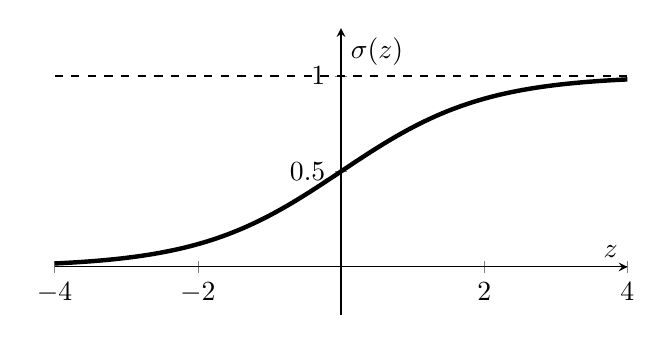
\begin{tikzpicture}
\begin{axis}[
  axis lines=middle,
  % axis equal image,
  scale only axis,
  width=0.6\textwidth,
  height=0.3\textwidth,
    xmin=-4, xmax=4,
    ymin=-0.25, ymax=1.25,
    xlabel={$z$}, ylabel={$\sigma(z)$},
]
\addplot [domain=-4:4, samples=100, ultra thick] {1/(1+exp(-x))};
\addplot [domain=-4:4, samples=2, dashed] {1};
\addplot [domain=-4:4, samples=2, dashed] {0};
\end{axis}
\end{tikzpicture}
\end{center}

\question{Convince yourself the output of $\sigma$ is always in the
  interval $(0, 1)$.  Why can't it equal 0 or equal 1?  For what value
of $z$ does $\sigma(z) = 0.5$?}

What does a linear logistic classifier (LLC) look like?   Let's consider the
simple case where $d = 1$, so our input points simply lie along the
$x$ axis.  The plot below shows LLCs for three different parameter
settings: $\sigma(10x + 1)$, $\sigma(-2x + 1)$, and $\sigma(2x - 3).$
\begin{center}
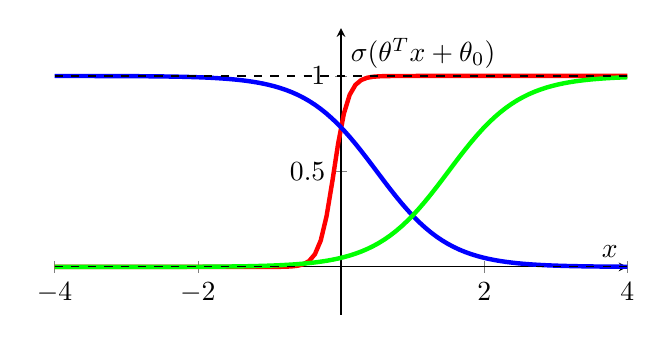
\begin{tikzpicture}
\begin{axis}[
  axis lines=middle,
  % axis equal image,
  scale only axis,
  width=0.6\textwidth,
  height=0.3\textwidth,
    xmin=-4, xmax=4,
    ymin=-0.25, ymax=1.25,
    xlabel={$x$}, ylabel={$\sigma(\theta^T x + \theta_0)$},
]
\addplot [domain=-4:4, samples=100, ultra thick, red] {1/(1+exp(-(10*x + 1)))};
\addplot [domain=-4:4, samples=100, ultra thick, blue] {1/(1+exp(-(-2*x
  + 1)))};
\addplot [domain=-4:4, samples=100, ultra thick, green] {1/(1+exp(-(2*x
  - 3)))};
\addplot [domain=-4:4, samples=2, dashed] {1};
\addplot [domain=-4:4, samples=2, dashed] {0};
\end{axis}
\end{tikzpicture}
\end{center}
\question{Which plot is which?  What governs the steepness of the
  curve?  What governs the $x$ value where the output is equal to
  0.5?}

But wait!  Remember that the definition of a classifier is that it's a mapping from $\R^d
\rightarrow \{-1, +1\}$ or to some other discrete set.  So, then, it
seems like an LLC is actually not a classifier! 

Given an LLC, with an output value in $(0, 1)$, what should we do if
we are forced to make a prediction in $\{+1, -1\}$?  A default answer
is to predict $+1$ if $\sigma(\theta^T x + \theta_0) > 0.5$ and $-1$
otherwise.  The value $0.5$ is sometimes called a {\em prediction
  threshold}.

In fact, for different problem settings, we might prefer to pick a
different prediction threshold.  The field of {\em decision theory}
considers how to make this choice from the perspective of Bayesian
reasoning.  For example, if the consequences of predicting $+1$ when
the answer should be $-1$ are much worse than the consequences of
predicting $-1$ when the answer should be $+1$, then we might set the
prediction threshold to be greater than $0.5$.

\question{Using a prediction threshold of 0.5, for what values of $x$
  do each of the LLCs shown in the figure above predict $+1$?}

% When $d = 2$, then our inputs $x$ lie in a two-dimensional space with
% axes $x_1$ and $x_2$, and the output of the LLC is a surface, as shown
% below, for $\theta = (1, 1), \theta_0 = 2$.

% \includegraphics[width=0.7\textwidth]{figures/logreg3d}

% \question{Convince yourself that the set of points for which
%   $\sigma(\theta^T x + \theta_0) = 0.5$, that is, the separator
%   between positive and negative predictions with prediction threshold
%   $0.5$ is a line in $(x_1, x_2)$ space. What particular line is it
%   for the case in the figure above?
%   How would the plot change for $\theta = (1, 1)$, but now
%   with $\theta_0 = -2$? For $\theta = (-1, -1), \theta_0 = 2$?}

A note about terminology and 
\anchorednote{notation.}
 {The notation within the algorithm above might be new to you:
  $\argmin{x} f(x)$ 
  means the value of $x$ for which $f(x)$ is the smallest.  Sometimes
  we write $\argmin{x \in {\cal X}} f(x)$ when we want to explicitly
  specify the set ${\cal X}$ of values of $x$ over which we want to
  minimize.}
The training data $\dataTrain$ is an input to the learning algorithm,
and the output of this learning algorithm will be a hypothesis $h$, where
$h$ has parameters $\theta$ and $\theta_{0}.$ 
In contrast to $\theta$ and $\theta_{0}$, the input $k$ is a 
parameter of the learning algorithm itself; such
parameters are often called {\em hyperparameters}.

\question{
What do you think will be observed for $\trainerr(h)$, where $h$ is the
hypothesis returned by \proc{Random-Linear-Classifier}, if this learning
algorithm is run multiple times? And as $k$ is increased? }

\question{
 What properties of $\dataTrain$ do you think will have an
effect on $\trainerr(h)$?
}

\subsubsection*{Loss function for logistic classifiers}

\label{logistic}
Recall that optimization is a key approach to solving machine learning
problems; this also applies to logistic regression, as we can see by
defining a lass function for this problem.  Recall that a common loss function
is the 0-1 loss, introduced in chapter \ref{intro}:
\[ L_{01}(h(x; \Theta), y) =
  \begin{cases}
    0 & \text{ if } y = h(x; \Theta)\\
    1 & \text{ otherwise}
  \end{cases}\;\;,
\]
which gives a value of 0 for a correct prediction, and a 1 for an
incorrect prediction.  In the case of linear separators, this becomes:
\[ L_{01}(h(x;\theta, \theta_0), y) =
  \begin{cases}
    0 & \text{ if } y(\theta^Tx + \theta_0) > 0 \\
    1 & \text{ otherwise}
  \end{cases}\;\;.
\]


%
For logistic regression, we have defined a class, LLC, of hypotheses whose outputs are in $(0, 1)$, 
but we have training data with $y$ values  in $\{+1, -1\}$.  How
can we define a loss function?  Intuitively, we would like to have
{\em low loss if we assign a low probability to the incorrect class.}
We'll define a loss function, called {\em negative log-likelihood} (NLL),
that does just this.  In  addition, it has the cool property that it
extends nicely to the case where we would like to classify our inputs
into more than two classes.

In order to simplify the description, we will assume that (or transform so that) the labels
in the training data are $y \in \{0, 1\}$, enabling them to be
interpreted as probabilities of being a member of the class of
interest.  \note{\bf Remember to be sure your $y$
  values have this form if you try to learn an LLC using NLL!|}
We would like to pick the parameters of our classifier to maximize the
probability assigned by the LCC to the correct $y$ values, as
specified in the training set.  Letting guess $\ex{g}{i} =
\sigma(\theta^T\ex{x}{i} + \theta_0)$, 
that probability is
\begin{equation*}
 \prod_{i = 1}^n \begin{cases} \ex{g}{i} & \text{if $\ex{y}{i} =
    1$}  \\ 1 - \ex{g}{i} & \text{otherwise}
\end{cases}\;\;,
\end{equation*}
under the assumption that our predictions are independent.  This can
be cleverly rewritten, when $\ex{y}{i} \in \{0, 1\}$, as
\begin{equation*}
 \prod_{i = 1}^n {\ex{g}{i}}^{\ex{y}{i}}(1 - \ex{g}{i})^{1 - \ex{y}{i}}\;\;.
\end{equation*}
\question{Be sure you can see why these two expressions are  the
  same.}

Now, because products are kind of hard to deal with, and because the
log function is monotonic, the $\theta, \theta_0$ that maximize the
log of this quantity will be the same  as the $\theta, \theta_0$ that
maximize the original, so we can try to maximize
\begin{equation*}
  \sum_{i = 1}^n  \left( {\ex{y}{i}}\log {\ex{g}{i}} +
            (1 - \ex{y}{i})\log(1 - \ex{g}{i})\right)\;\;. 
\end{equation*}
We can turn the maximization problem above into a minimization problem by taking the negative
of the above expression, and write in terms of minimizing a loss
\begin{equation*}
 \sum_{i = 1}^n \mathcal{L}_\text{nll}(\ex{g}{i}, \ex{y}{i})
\end{equation*}
where $\mathcal{L}_\text{nll}$ is the {\em negative log-likelihood}
loss function:
\begin{equation*}
\mathcal{L}_\text{nll}(\text{guess},\text{actual}) = 
-\left(\text{actual}\cdot \log (\text{guess}) + (1 - \text{actual})\cdot\log (1 -
  \text{guess})\right) \;\;.
\end{equation*}
This loss function is also sometimes referred to as the {\em log loss}
or {\em cross entropy}. \note{You can use any base for the logarithm
  and it won't make any real difference.  If we ask you for numbers,
  use log base $e$.}


% \qn{state problem statement and setup --> reduce to optimization problem.}



\section{Evaluate a learning algorithm}

% \begin{itemize}
%     \item Error decomposition
%     \item Overfitting, underfitting
% \end{itemize}
% % Estimator, bias, variance, MSE → underfitting, overfitting
% \subsection{Evaluating a learning algorithm}
How should we evaluate the performance of a {\em classifier} $h$?   The best
method is to measure {\em test error} on data that was not used to
train it. 

How should we evaluate the performance of a {\em learning algorithm}?
This is trickier.  There are many potential sources of variability in
the possible result of computing test error on a learned hypothesis $h$:
\begin{itemize}
\item Which particular {\em training examples} occurred in $\dataTrain$
\item Which particular {\em testing examples} occurred in $\dataTest$
\item Randomization inside the learning {\em algorithm} itself
\end{itemize}
Generally, we would like to execute the following process multiple
times: 
\begin{itemize}
\item Train on a new training set
\item Evaluate resulting $h$ on a testing set {\em that does not
    overlap the training set}
\end{itemize}
Doing this multiple times controls for possible poor choices of
training set or unfortunate randomization inside the algorithm itself.

One concern is that we might need a lot of data to do this, and in
many applications data is expensive or difficult to acquire. We can 
re-use data with {\em{cross validation}} (but it's harder to do theoretical
analysis).  \\
\begin{codebox}
  \Procname{$\proc{Cross-Validate}(\data, k)$}
  \li divide $\data$ into $k$ chunks $\data_1, \data_2, \ldots \data_k$ (of roughly equal size)
  \li \For $i \gets 1$ \To $k$
  \li   \Do
          train $h_i$ on $\data \setminus \data_i$ (withholding chunk $\data_i$)
  \li     compute ``test'' error $\mathcal{E}_i (h_i)$ on withheld data $\data_i$
        \End
  \li \Return $\frac{1}{k} \sum_{i=1}^k \mathcal{E}_i (h_i)$
\end{codebox}

It's very important to understand that cross-validation neither
delivers nor evaluates a single particular hypothesis $h$.  It
evaluates the {\em algorithm} that produces hypotheses.

\end{document}